\documentclass{standalone}
\usepackage{tikz}
\begin{document}
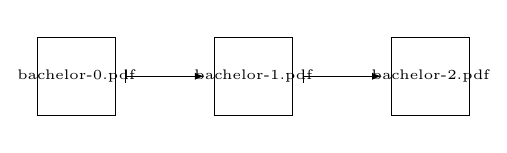
\begin{tikzpicture}
  \pgfdeclareimage[height=1cm]{ba}{bachelor-0.pdf}
  \pgfdeclareimage[height=1cm]{bb}{bachelor-1.pdf}
  \pgfdeclareimage[height=1cm]{bc}{bachelor-2.pdf}

  \pgfmathsetmacro{\kx}{2.25}

  \node (a) at (-\kx,0) {\pgfuseimage{ba}};
  \node (b) at (0,0) {\pgfuseimage{bb}};
  \node (c) at (\kx,0) {\pgfuseimage{bc}};

  \draw [very thin,|-latex] (a) -- (b);
  \draw [very thin,|-latex] (b) -- (c);

  % \node (rkd) at (\kx,-\ky) {\pgfuseimage{rkd}};
  % \node (rke) at (-\kx,-2*\ky) {\pgfuseimage{rke}};
  % \node (rkf) at (\kx,-2*\ky) {\pgfuseimage{rkf}};

  % % x coordinate for drawing arrows in the center
  % \pgfmathsetmacro{\xc}{.5}

  % % And for the sides
  % % X coordinate for leaving on the right side
  % \pgfmathsetmacro{\xlr}{5.25}

  % % Coordinates for right bend
  % \pgfmathsetmacro{\xrb}{5.5}

  % % coordinates for left bend
  % \pgfmathsetmacro{\xlb}{-5.5}

  % % Coordinates for incoming on the left side
  % \pgfmathsetmacro{\xil}{-5}

  % \foreach \y in {0,-\ky}{
  %   \draw[|-latex, densely dotted] (-\xc, \y) -- (\xc, \y);
  %   \draw[|-latex, densely dotted] (\xlr, \y) -- (\xrb, \y) --
  %   (\xrb, \y-\ky/2) -- (\xlb, \y-\ky/2) -- (\xlb, \y-\ky) -- (\xil,
  %   \y-\ky);
  % }

  % \draw[|-latex, densely dotted] (-\xc, -2*\ky) -- (\xc, -2*\ky);
\end{tikzpicture}
\end{document}
